% RESULTS %

%\Section{Results}\label{sec:results}
The results of the different models are presented individually and compared by the mean squared error to emphasize 
large errors over small ones.

\subsection{Linear Regression}
\subsection{CNN}
\subsection{RNN}
      RNN is trained with the extracted and preprocessed data feature acquired in the experiment (depth at maximum intensity) from the OCT depth scan as input to predict the force acting at the needle, as there exist a direct relationship between force data (measured using a force sensor) and the OCT image. This is a supervised learning, as force data from the force sensor is initially used for the training of RNN. Once the training is completed, one can predict the force acting at the needle with the OCT data alone without the help of force sensor.
      \begin{figure}
    \centering
    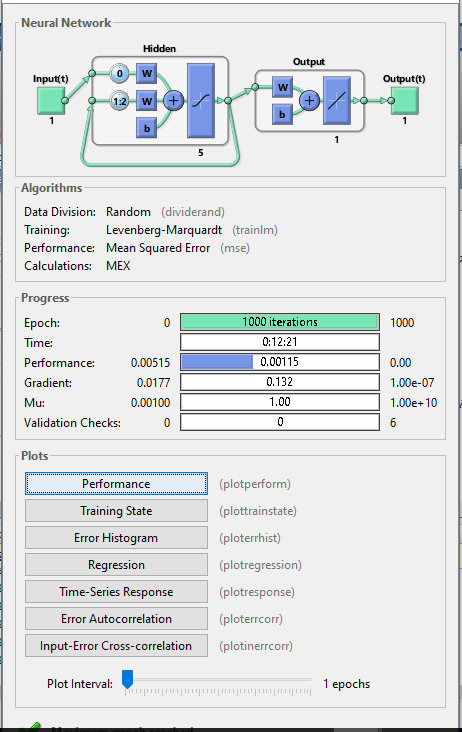
\includegraphics[width=0.9\textwidth]{RNN-toolbox.png}
    \caption{RNN toolbox in MATLAB showing the progress after 1000 iterations}
    \label{fig:RNN toolbox}
\end{figure}
      
      Here, RNN is trained using Neural Network toolbox in MATLAB. A recurrent net layer is created with one input layer, one output layer and 5 hidden layers and with the training function trainlm. As you can see in fig. the RNN is trained with the training function Levenberg-Marquardt and the performance is measured by mean squared error. Training is started with a mean squared error of 0.00515 and ended up with 0.00115 at the end of 1000 iterations. Validation is automatically taken care in the Neural network training toolbox itself. Once the training is done, the trained model is saved for testing. 
      
      RNN trained data is now used to predict the force value from the given OCT data. The input OCT data for testing is acquired from the experimental data and the output from the RNN is compared with the force sensor value and the performance is measured as root mean square and is summarized in the table below for different input conditions (linear & stepwise movement of needle against metal and Phantom). 
    
\begin{figure}
    \centering
    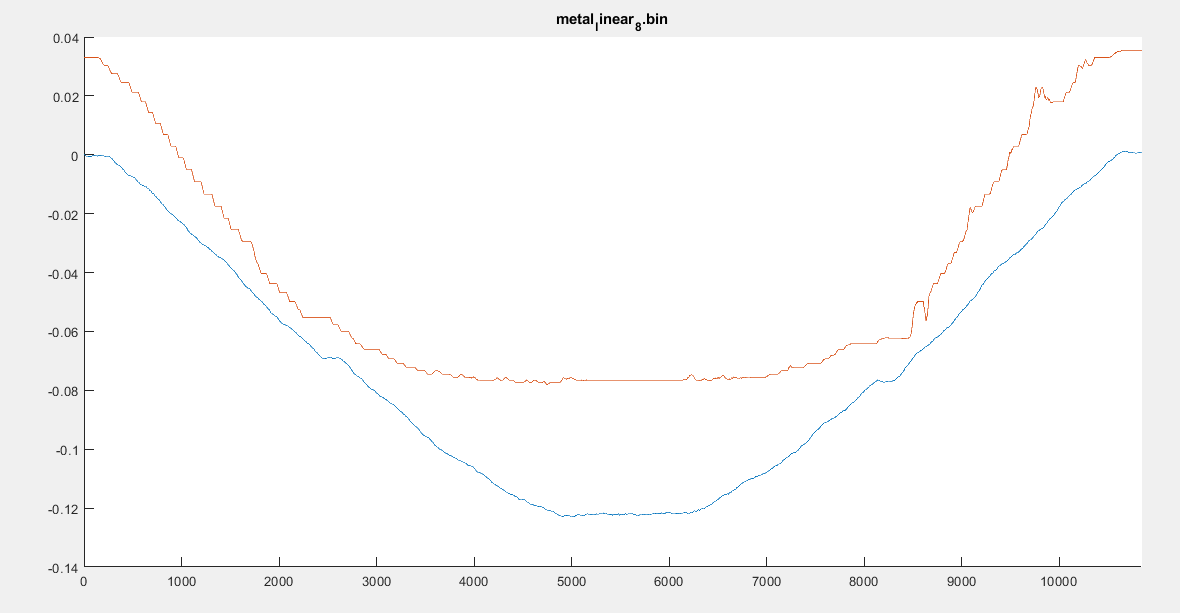
\includegraphics[width=0.9\textwidth]{metallinear8.png}
    \caption{Force prediction and actual force for the poking the needle against metal linearly}
    \label{fig:metallinear8}
\end{figure}


\begin{figure}
    \centering
    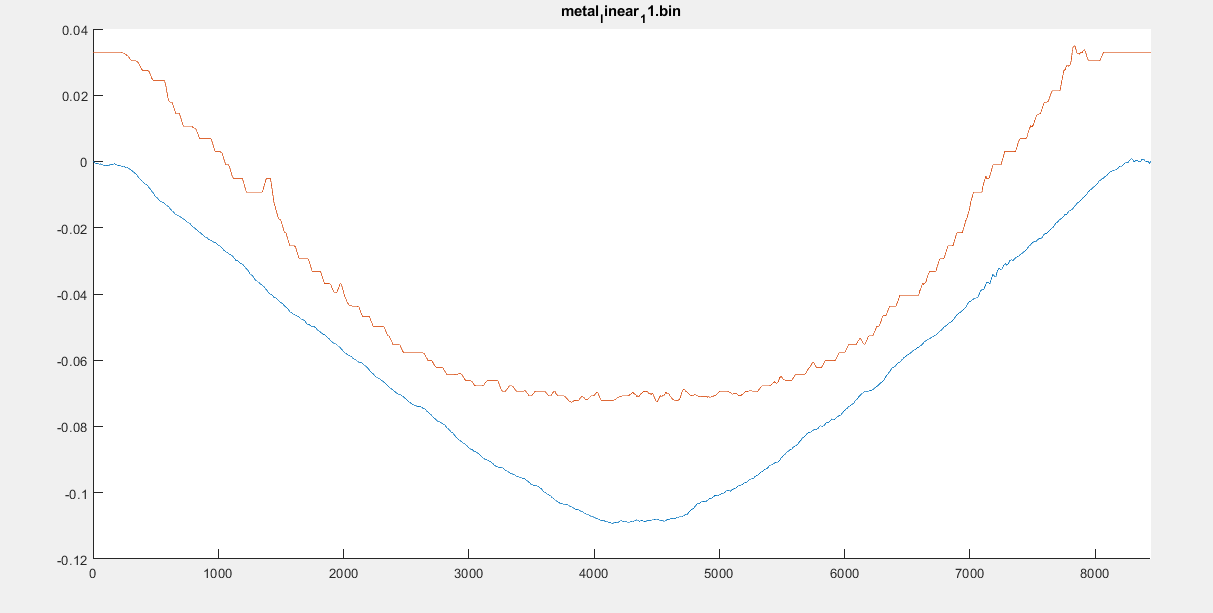
\includegraphics[width=0.9\textwidth]{metallinear11.png}
    \caption{Force prediction and actual force for the poking the needle against metal linearly}
    \label{fig:metallinear11}
\end{figure}

\begin{figure}
    \centering
    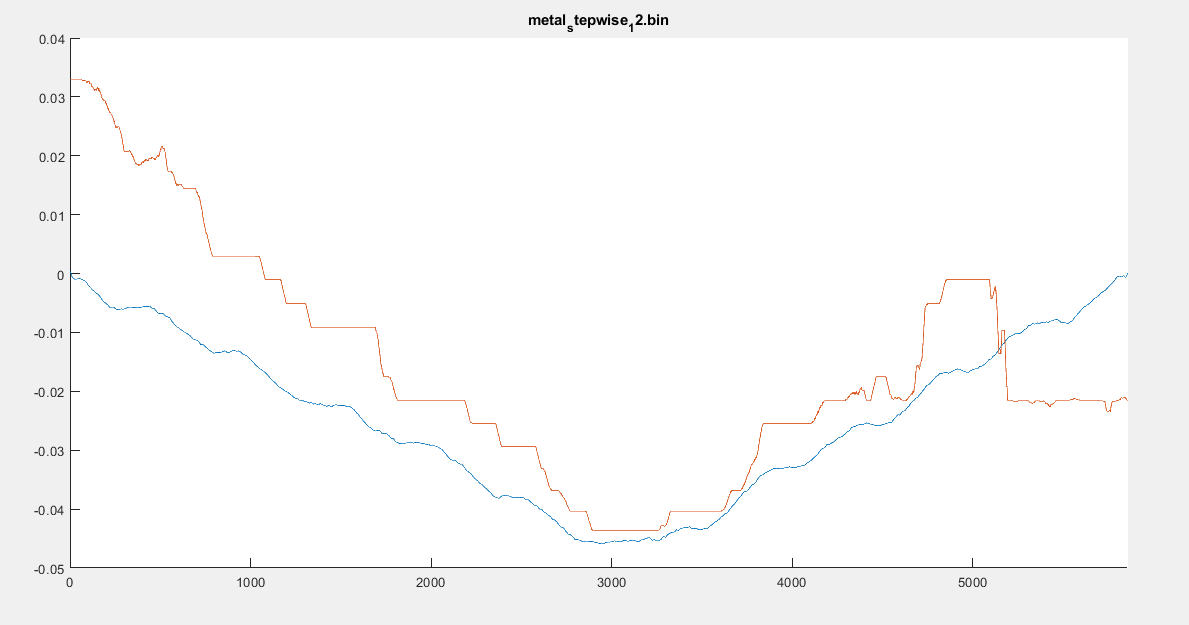
\includegraphics[width=0.9\textwidth]{metalstepwise12.png}
    \caption{Force prediction and actual force for the poking the needle against metal stepwise}
    \label{fig:metalstepwise12}
\end{figure}

\begin{figure}
    \centering
    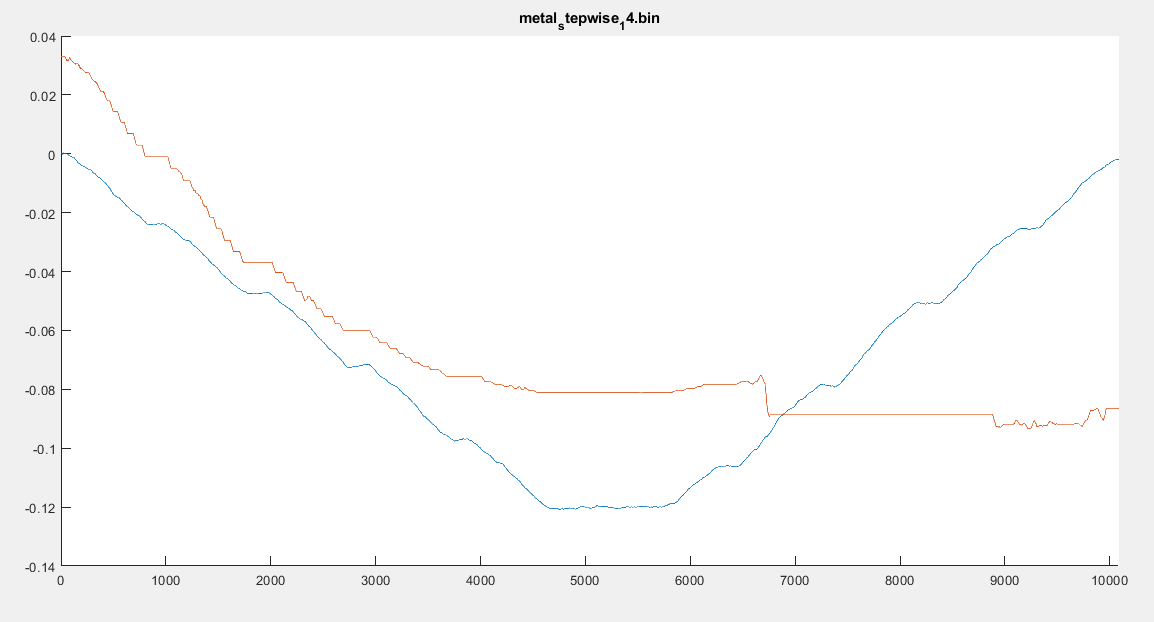
\includegraphics[width=0.9\textwidth]{metalstepwise14.png}
    \caption{Force prediction and actual force for the poking the needle against metal stepwise}
    \label{fig:metalstepwise14}
\end{figure}

\begin{figure}
    \centering
    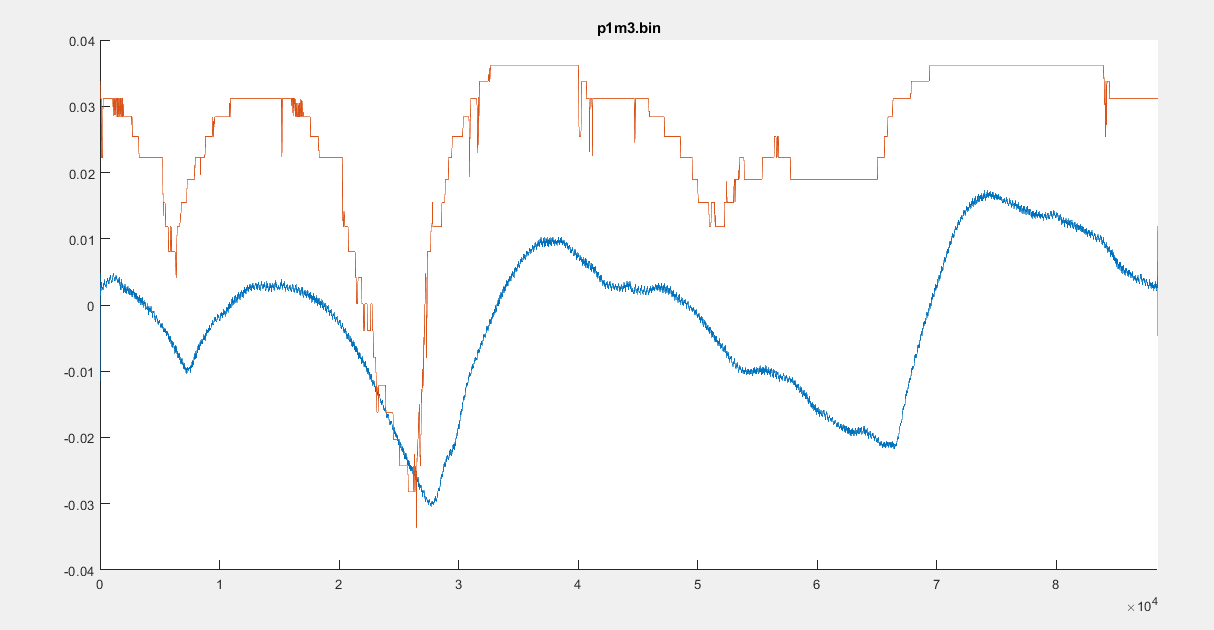
\includegraphics[width=0.9\textwidth]{p1m3.png}
    \caption{Force prediction and actual force for the poking the needle against phantom}
    \label{fig:Phantom}
\end{figure}
      
      
      
\subsection{Comparison}
